\label{app:heatTransVac}

An important factor in determining the temperatures reached within accelerator components is the rate of energy transfer from the internal components to the surrounding vacuum tank. in particular the high vacuum required in accelerator operation means that the transfer of energy becomes dominated by conduction and radiative transfer due to the absence of a medium convection. Depending on the structure conduction of heat between components in contact may not be well defined, and radiative transfer can be strongly affected by the surface emissivities of the components, particularly a concern due to the polishing of metallic surfaces for vacuum compatability which tends to leave the surfaces with a relatively low thermal emissivity ($\epsilon \approx 0.1$).

Here we shall briefly cover passive cooling within accelerator structures, discussing convection, conduction (including the case of near-field IR tunnelling) and radiative transfer.

\section{Convection}

The majority of accelerator components are under extremely high vacuum to support the circulating particle beam and thus there is little to any medium in which convection currents may flow. In this case the heat transfer by vacuum by means of convection is negligible.

\section{Conduction}

Conduction between components in an accelerator device can be varied in their degree of contact. Components that are afixed by some form of bonding (welding, brazing) have a well defined heat transfer by conduction due to the good physical bond between them. However components that are afixed by contact pressure (i.e. pushed by screw/nut, held by a casing/housing or just under the weight of gravity) may not have good or well-defined thermal contact with one another. This is due to the variation in the thermal conductivity between the two components depending on contact pressure, surface flatness, and the cleanliness of the surface (generally not a signficant factor in high vacuum quality finishes).

In particular some components may be highly sensitive to strongly exerted forces to improve contact pressure due to brittleness or mechanical weakness. In this case the heat transfer by conduction is not necessarily significant or simply represented.

\section{Radiation}

Radiation is very well defined in terms of heat radiation transfer within a vacuum. Two important factors in determining the thermal conductivity due to thermal radiation between two components are the thermal emissivity of the materials and the ratio visible surface areas of the two materials. This effect is seen in Fig.~\ref{fig:powTransRadSurfEmis}, it which is can be seen in the case of where the emissivity of the absorbing material is low ($< 0.2$), small changes in the emissivity can greatly increase or decrease the rate of power transfer. This is exacerbated the smaller the ratio of the surface areas between the emitting and absorbing components.

\begin{figure}
\begin{center}
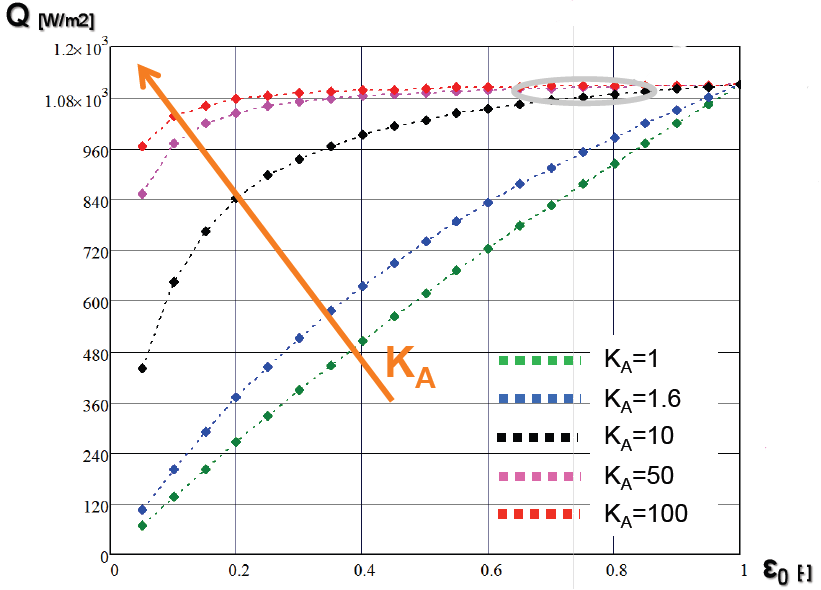
\includegraphics[width=0.55\textwidth]{appendices/figures/powTransRadSurEmis.png}
\end{center}
\caption{The power transfer between two surfaces by radiative heat transfer as a function of emissitivity of the absorbing component and the ratio of the visible surface areas of the components. K$_{A}$ is the ratio of the surface of the absorbing component and the emitting component. Figure produced by Garlasche et al \cite{Garlasche:heatTransfer}.}
\label{fig:powTransRadSurfEmis}
\end{figure}

It can be seen that for components that may be exposed to dangerous heat loads (i.e. ferrites, thermal sensitive equipment), heat transfer by radiation may be improved by the increasing the emissivity of surrounding components, and making sure it is thermally visible to a large surrounding area.

\subsection{Near-field radiation}

In the case where two components are exceptionally close to one another a curious phenomena known as radiative tunnelling. This effect on the thermal transfer is shown in Fig.~\ref{fig:irTun}, where is can be seen that there is a region between the radiation dominated heat transfer and the conduction dominated transfer as two objects are moved closer together where the thermal conductivity greatly increases, but before the components are in physical contact. This is significant as it may be exceptionally beneficial to the heat evacuation in of components that are in close proximity to surrounding components, but where the physical contact is not good, such as the case where ferrites are held in a casing, which due to their brittleness may not have a large physical force exuded on them.

\begin{figure}
\begin{center}
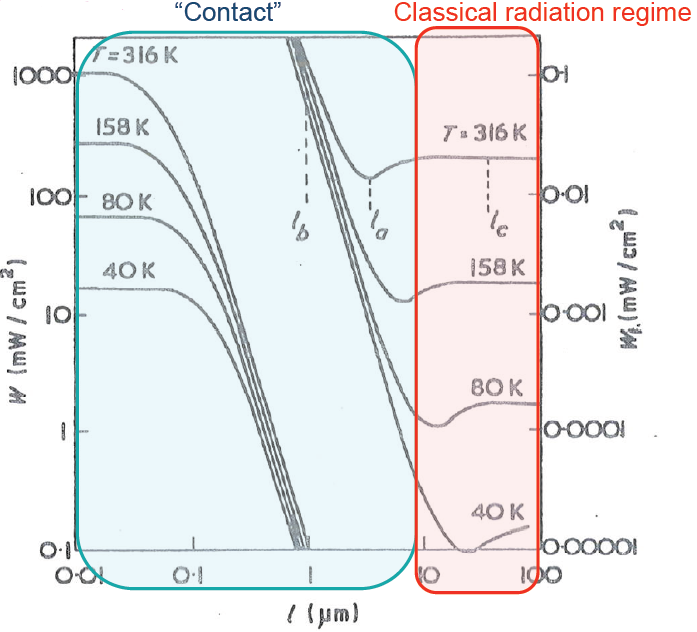
\includegraphics[width=0.55\textwidth]{appendices/figures/irTunnelling.png}
\end{center}
\caption{An illustration of the change between the two regimes of thermal transfer by radiation and by conduction as the distance between two surfaces is reduced. It can be seen that there is a period between radiation and the beginning of transfer by contact where-in the rate of thermal transfer greatly increases. This is due to an effect known as radiative tunnelling \cite{Hargreaves:IRTunnel}.}
\label{fig:irTun}
\end{figure}
